\chapter{Canonical Quantization}

    The main reference for this chapter is~\citet{peskin_introduction_1995}.

\section{Klein--Gordon field}\index{Klein--Gordon equation}
\subsection{Lagrangian and Hamiltonian}

    The `simplest' Lagrangian (density) is given by
    \begin{gather}
        \label{qft:klein_gordon_lagrangian}
        \mathcal{L} = \frac{1}{2}\partial_\mu\phi\partial^\mu\phi - \frac{1}{2}m^2\phi^2\,.
    \end{gather}
    Using the principle of least action, the following Euler--Lagrange equation is obtained:
    \begin{gather}
        \left(\partial^\mu\partial_\mu + m^2\right)\phi = 0\,.
    \end{gather}
    This can be rewritten using the \textbf{d'Alembertian} $\Box = \partial_\mu\partial^\mu$:\index{d'Alembert!operator}
    \nomenclature[O_dAl]{$\Box$}{d'Alembert operator}
    \begin{gather}
        \label{qft:klein_gordon_equation}
        (\Box+m^2)\phi = 0\,.
    \end{gather}
    This equation is called the \textbf{Klein--Gordon equation}. In the limit $m\rightarrow0$ this equation reduces to the well-known wave equation.

    From the Lagrangian~\eqref{qft:klein_gordon_lagrangian}, one can also derive a Hamiltonian function using \cref{lagrange:conjugate_momentum} and \cref{lagrange:hamiltonian}:
    \begin{gather}
        \label{qft:klein_gordon_hamiltonian}
        H = \frac{1}{2}\Int_{\mathbb{R}^3}\left[\pi^2(x) + (\nabla\phi(x))^2 + m^2\phi^2(x)\right]\,d^3x\,.
    \end{gather}

\subsection{Raising and lowering operators}

    Fourier transforming the scalar field $\phi(\mathbf{x})$ in momentum space and inserting it into the Klein--Gordon equation gives
    \begin{gather}
        \left(\partial_t^2+p^2+m^2\right)\phi(\mathbf{p}) = 0\,.
    \end{gather}
    This is the equation for a simple harmonic oscillator with frequency $\omega = \sqrt{p^2+m^2}$.

    Analogous to ordinary quantum mechanics, raising and lowering operators $a_{\vector{p}}^\dag$ and $a_{\vector{p}}$ can be defined such that
    \begin{align}
        \phi(\vector{x}) &= \Iiint\frac{d^3p}{(2\pi)^{3/2}}\frac{1}{\sqrt{2\omega_{\vector{p}}}}\left(a_{\vector{p}}e^{i\vector{p}\cdot\vector{x}} + a_{\vector{p}}^\dag e^{-i\vector{p}\cdot\vector{x}}\right)\,,\label{qft:phi}\\
        \pi(\vector{x}) &= \Iiint\frac{d^3p}{(2\pi)^{3/2}}(-i)\sqrt{\frac{\omega_{\vector{p}}}{2}}\left(a_{\vector{p}}e^{i\vector{p}\cdot\vector{x}} - a_{\vector{p}}^\dag e^{-i\vector{p}\cdot\vector{x}}\right)\,.
    \end{align}
    An equivalent definition is obtained by performing the transformation $\vector{p}\longrightarrow-\vector{p}$ in the second term of $\phi(\vector{x})$ and $\pi(\vector{x})$:
    \begin{align}
        \phi(\vector{x}) &= \Iiint\frac{d^3p}{(2\pi)^{3/2}}\frac{1}{\sqrt{2\omega_{\vector{p}}}}\left(a_{\vector{p}} + a_{-\vector{p}}^\dag\right)e^{i\vector{p}\cdot\vector{x}}\,,\\
        \pi(\vector{x}) &= \Iiint\frac{d^3p}{(2\pi)^{3/2}}(-i)\sqrt{\frac{\omega_{\vector{p}}}{2}}\left(a_{\vector{p}} - a_{-\vector{p}}^\dag\right)e^{i\vector{p}\cdot\vector{x}}\,.
    \end{align}

    When the commutation relation
    \begin{gather}
        \label{qft:ladder_comutation}
        [a_{\vector{p}},a_{\vector{q}}^\dag] := \delta(\vector{p}-\vector{q})
    \end{gather}
    is imposed, the following commutation relation for the scalar field and its conjugate momentum is obtained:
    \begin{gather}
        [\phi(\vector{x}),\pi(\vector{y})] = i\delta(\vector{x} - \vector{y})\,.
    \end{gather}
    Now, the Hamiltonian can be calculated explicitly:
    \begin{gather}
        \label{qft:Klein_gordon_hamiltonian}
        H = \Int\frac{d^3p}{(2\pi)^3}\omega_{\vector{p}}\left(a_{\vector{p}}^\dag a_{\vector{p}} + \frac{1}{2}[a_{\vector{p}},a_{\vector{p}}^\dag]\right)\,.
    \end{gather}
    However, it is clear from \cref{qft:ladder_comutation} that the second term in this integral diverges. There are two reasons for this divergence. First, space is infinite, i.e.~the $d^3x$ integral in \cref{qft:klein_gordon_hamiltonian} diverges. This problem can be resolved by restricting the system to a (finite) part of space or by considering the energy density instead of the energy itself. Second, by including very large values for $p$ in the integral, a parameter range is explored where the theory is likely to break down. To resolve this problem a  `high $p$'-cut-off should be introduced. A more practical solution, however, is to note that only energy differences are physical and so one can simply drop the second term altogether as it is merely a `constant' (albeit an infinite one).

    A corollary of \cref{qft:Klein_gordon_hamiltonian} together with the canonical commutation relations is
    \begin{align}
        [H,a_{\vector{p}}^\dag] &= \omega_pa_{\vector{p}}^\dag\,,\\
        [H,a_{\vector{p}}] &= -\omega_pa_{\vector{p}}\,.
    \end{align}
    As was the case for the quantum harmonic oscillator, the creation and annihilation operators deserve their names and one can write:
    \begin{gather}
        |\vector{k}_1,\ldots,\vector{k}_n\rangle = a^\dag(\vector{k}_1)\cdots a^\dag(\vector{k}_n)|0\rangle\,.
    \end{gather}
    Furthermore, this equation together with the canonical commutation relations imply that the Klein--Gordon fields are bosonic fields. This way of generating the full Hilbert (in fact Fock) state space is axiomatized by the GNS construction (\cref{operators:gns}), where the vacuum plays the role of cyclic vector.

\subsection{Scalar propagator}

    \newformula{Pauli--Jordan function}{\index{Pauli--Jordan function}
        \begin{gather}
            i\Delta(\mathbf{x}-\mathbf{y}) := i[\phi(\mathbf{x}),\phi(\mathbf{y})] = \Int\frac{d^3p}{(2\pi)^3}\frac{1}{2\omega_{\mathbf{x}}}\left(e^{-i\mathbf{p}\cdot(\mathbf{x}-\mathbf{y})} - e^{i\mathbf{p}\cdot(\mathbf{x}-\mathbf{y})}\right)
        \end{gather}
        In the case that $x^0=y^0$ (ETCR) or $(\mathbf{x}-\mathbf{y})^2 < 0$ (spacelike curves), the Pauli--Jordan function is identically 0. (See also the \textit{axiom of microcausality} (\cref{aqft:microcausality})).
    }

\subsection{Normalization constant}

    By \cref{distribution:delta_of_function}, the delta function $\delta^{(3)}(\vector{p}-\vector{q})$ transforms as $\delta^{(3)}(\Lambda\vector{p} - \Lambda\vector{q})\frac{\Lambda E}{E}$ under a general Lorentz boost $\Lambda$. Although this is clearly not Lorentz invariant, the quantity $E_{\mathbf{x}}\delta^{(3)}(\vector{p}-\vector{q})$ can be seen to be invariant. From this observation it follows that the correct normalization in the momentum representation becomes
    \begin{gather}
        |\mathbf{p}\rangle = \sqrt{2E_{\mathbf{x}}}a_{\mathbf{p}}^\dag|0\rangle
    \end{gather}
    and, hence,
    \begin{gather}
        \langle\mathbf{p}\mid\mathbf{q}\rangle = 2E_{\mathbf{x}}(2\pi)^3\delta^{(3)}(\vector{p}-\vector{q})\,,
    \end{gather}
    where the constants are a matter of convention to cancel the constants in \cref{qft:phi}.

\subsection{Invariant integration measure}

    The factor $2E_p$ does not only occur in the normalization conditions. To find a Lorentz invariant integration measure in spacetime, the following integral can be studied:
    \begin{gather}
        \Int\frac{d^3p}{2E_p} = \left.\Int\delta(p^2-m^2)\,d^4p\,\right|_{p^0>0}\,.
    \end{gather}
    By using this measure, it is ensured that the integral of any Lorentz invariant function is again Lorentz invariant.
    \begin{example}[One-particle identity operator]\index{identity!operator}
        \begin{gather}
            \mathbbm{1} := \Int\frac{d^3p}{2E_p}|\mathbf{p}\rangle\langle\mathbf{p}|
        \end{gather}
    \end{example}

\section{Contractions and Wick's theorem}
\subsection{Bosonic fields}

    In the following definitions, (field) operators will be decomposed as \[\phi = \phi^{(+)} + \phi^{(-)}\,,\] where the + symbol denotes the `positive frequency' part, i.e.~the part consisting of annihilation operators. The `negative frequency' part is defined analogously. This terminology stems from the classic Fourier integral. By looking at \cref{qft:phi} and remembering that the $(1,3)$-signature is adopted,the annihilators can be seen to always occur together with a positive frequency exponential.

    \newdef{Contraction for neutral bosonic fields}{\index{contraction}
        \begin{gather}
            \contraction{}{\phi}{(\mathbf{x})}{\phi}\phi(\mathbf{x})\phi(\mathbf{y}) :=
            \begin{cases}
                [\phi(\mathbf{x})^{(+)},\phi(\mathbf{y})^{(-)}]&x^0>y^0\\
                [\phi(\mathbf{y})^{(+)},\phi(\mathbf{x})^{(-)}]&y^0>x^0
            \end{cases}
        \end{gather}
    }
    \newformula{Feynman propagator}{\index{Feynman!propagator}\label{qft:feynman_propagator_contraction}
        \begin{gather}
            i\Delta_F(\mathbf{x}-\mathbf{y}) := \contraction{}{\phi}{(\mathbf{x})}{\phi}\phi(\mathbf{x})\phi(\mathbf{y}) := i\lim_{\varepsilon\rightarrow 0^+}\Int\frac{d^4p}{(2\pi)^4}\frac{e^{-i\mathbf{p}\cdot(\mathbf{x}-\mathbf{y})}}{p^2 - m^2 + i\varepsilon}
        \end{gather}
    }

    \newdef{Contraction for charged bosonic fields}{
        \begin{gather}
            \contraction{}{\phi}{(\mathbf{x})}{\overline\phi}\phi(\mathbf{x})\overline\phi(\mathbf{y}) :=
            \begin{cases}
                [\phi(\mathbf{x})^{(+)},\overline\phi(\mathbf{y})^{(-)}]&x^0>y^0\\
                [\phi(\mathbf{y})^{(+)},\overline\phi(\mathbf{x})^{(-)}]&y^0>x^0
            \end{cases}
        \end{gather}
    }

    \newdef{Normal ordering}{\index{normal!ordering}
        The normal ordering $\mathcal{N}$, often denoted by colons $:\ \ :$, of a sequence of field operators is defined as the permuted sequence in which all annihilation operators appear on the right of the creation operators, e.g.: \[\mathcal{N}\bigl(\phi(\mathbf{x})\phi^\dag(\mathbf{y})\phi(\mathbf{z})\bigr) = \phi^\dag(\mathbf{y})\phi(\mathbf{x})\phi(\mathbf{z})\,.\] Note that the normal ordering operator is not a morphism between CCR-algebras since this would lead to a contradiction: \[b_ib_j^\dag = b_j^\dag b_i + \delta_{ij}\implies\mathcal{N}(b_ib_j^\dag) = \mathcal{N}(b_j^\dag b_i+\delta_{ij}) = \mathcal{N}(b_j^\dag b_i) + \delta_{ij}\implies\delta_{ij}=0\,.\] The solution is given by the fact that inside the normal ordering all operators commute and, hence, this ordering can be axiomatized as an algebra morphism $\mathcal{N}:\Sym^\bullet A\rightarrow A$, where $A$ is the CCR-algebra of the theory (see~\citet{miwa_solitons_2000}).

        @@ IS THIS REFERENCE CORRECT? @@
    }
    \begin{property}
        From this definition, it immediately follows that the vacuum expectation value of a normal ordered sequence is 0.
    \end{property}

    \newformula{Wick's theorem for bosonic fields}{\index{Wick!theorem for time-ordered integrals}
        \begin{gather}
            \mathcal{T}\bigl(\phi(\mathbf{x}_1)\cdots\phi(\mathbf{x}_n)\bigr) = \mathcal{N}\bigl(\phi(\mathbf{x}_1)\cdots\phi(\mathbf{x}_n) + \text{all possible contractions}\bigr)
        \end{gather}
        When acting with such a time-ordered product on the vacuum, this theorem implies that only fully contracted terms will remain. Moreover, by \cref{qft:feynman_propagator_contraction}, every such action can be expressed solely in terms of propagators.
    }

    \begin{remark}
        In the case of charged bosons, only contractions of the form $\contraction{}{\phi}{(\mathbf{x})}{\overline\phi}\phi(\mathbf{x})\overline\phi(\mathbf{y})$ will remain because $[a,b^+]=0$.
    \end{remark}

    \begin{result}
        \begin{gather}
            \contraction{}{\phi}{(\mathbf{x})}{\phi}\phi(\mathbf{x})\phi(\mathbf{y}) = \mathcal{T}\bigl(\phi(\mathbf{x})\phi(\mathbf{y})\bigr) - \mathcal{N}\bigl(\phi(\mathbf{x})\phi(\mathbf{y})\bigr)
        \end{gather}
    \end{result}

    Wick's theorem has an analogue in probability theory.
    \begin{theorem}[Isserlis]\index{Isserlis}
        Let $X_1,\ldots,X_n$ be a set of random variables following a multinormal distribution with mean 0.
        \begin{gather}
            \expect{X_1\cdots X_n} = \sum_{\sigma\in P_{n,2}}\prod_{\{i,j\}\in\sigma}\expect{X_iX_j}\,,
        \end{gather}
        where $P_{n,2}$ denotes the set of binary partitions of $\{1,\ldots,n\}$. Because the mean of the distribution is zero, this expression is equal to
        \begin{gather}
            \expect{X_1\cdots X_n} = \sum_{\sigma\in P_{n,2}}\prod_{\{i,j\}\in\sigma}\mathrm{cov}[X_iX_j]\,.
        \end{gather}
    \end{theorem}

\subsection{Fermionic fields}

    \newdef{Contraction}{
        \begin{gather}
            \contraction{}{\psi}{(\mathbf{x})}{\overline\psi}\psi(\mathbf{x})\overline\psi(\mathbf{y}) :=
            \begin{cases}
                \{\psi(\mathbf{x})^{(+)},\overline\psi(\mathbf{y})^{(-)}\}_+&x^0>y^0\\
                -\{\psi(\mathbf{y})^{(+)},\overline\psi(\mathbf{x})^{(-)}\}_+&y^0>x^0
            \end{cases}
        \end{gather}
    }
    \begin{remark}
        Only contractions of the form $\contraction{}{\psi}{(\mathbf{x})}{\overline\psi}\psi(\mathbf{x})\overline\psi(\mathbf{y})$ will remain because $\{a,b^\dag\}_+=0$.
    \end{remark}

    \newformula{Feynman propagator}{\index{Feynman!propagator}
        \begin{gather}
            i\Delta_F(\mathbf{x}-\mathbf{y}) := \contraction{}{\psi}{(\mathbf{x})}{\overline\psi}\psi(\mathbf{x})\overline\psi(\mathbf{y}) := i\lim_{\varepsilon\rightarrow 0^+}\Int\frac{d^4\mathbf{p}}{(2\pi)^4}\frac{\slashed{\mathbf{p}} + m}{p^2 - m^2 + i\varepsilon}e^{-i\mathbf{p}\cdot(\mathbf{x}-\mathbf{y})}
        \end{gather}
    }

    \begin{remark}[Normal ordering]
        One should take into account the Fermi-Dirac statistics when permuting fermionic field operators under a normal ordering. A general factor $\sgn(\sigma)$, where $\sigma$ is the permutation of the operators, will arise in every term, e.g.: \[\mathcal{N}\bigl(\psi(\mathbf{x})\overline\psi(\mathbf{y})\psi(\mathbf{z})\bigr) = -\overline\psi(\mathbf{y})\psi(\mathbf{x})\psi(\mathbf{z})\] A similar remark should be made for the time-ordering operator $\mathcal{T}$. As was the case for bosonic theories one should pay attention to the nature of the normal ordering. It is not a morphism between CAR-algebras, but instead it is an algebra morphism between a free (odd) algebra and a CAR-algebra.
    \end{remark}

\section{Feynman rules}
\subsection{Scalar theory}

    By expanding the correlation functions in perturbation theory and applying Wick's theorem, one can rewrite every term using the following dictionary for Feynman diagrams (for these rules it is assumed that every coupling constant in the Lagrangian is divided by the necessary permutation factors, e.g.~in $\phi^4$-theory it is assumed that the constant is of the form $\lambda/4!$):
    \begin{itemize}
        \item Propagator $\Delta_F(\mathbf{x}-\mathbf{y})$:
            \begin{gather*}
                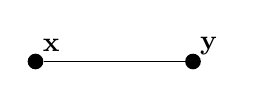
\begin{tikzpicture}
                    \node (labx) at (0.2,0.2) {$\mathbf{x}$};
                    \node (laby) at (2.2,0.2) {$\mathbf{y}$};
                    \node (x) at (0,0) [circle,fill,inner sep=2pt] {};
                    \node (y) at (2,0) [circle,fill,inner sep=2pt] {};
                    \draw (x) -- (y);
                \end{tikzpicture}
            \end{gather*}
        \item Interaction vertex\footnote{Four legs were drawn as an example but this can be generalized to any order of interaction term.} $-i\lambda\int d^4z$:
            \begin{gather*}
                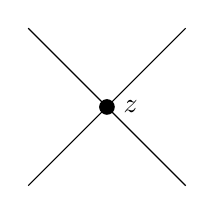
\begin{tikzpicture}
                    \node (z) at (0.3,0) {$z$};
                    \node (x) at (0,0) [circle,fill,inner sep=2pt] {};
                    \draw (-1,-1) -- (1,1);
                    \draw (-1,1) -- (1,-1);
                \end{tikzpicture}
            \end{gather*}
    \end{itemize}
    The main idea behind these rules is to draw all possible diagrams consistent with the given interaction Lagrangian and translate them into analytic expressions. However, to obtain the correct normalization, one should take the following remark into account.
    \begin{remark}\index{symmetry!factor}
        Symmetry factors of diagrams should be accounted for in analytic expressions. As an example consider the following vacuum bubble:
        \begin{gather*}
            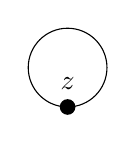
\begin{tikzpicture}
                \node (z) at (0, 0.3) {$z$};
                \node (x) at (0,0) [circle,fill,inner sep=2pt] {};
                \draw (0,0.5) circle (0.5);
            \end{tikzpicture}
        \end{gather*}
        Because the two legs can be interchanged, this diagram has \textbf{symmetry factor} 2 and, hence, it gives the analytic expression $-\frac{i\lambda}{2}\int d^4z\,\Delta_F(\mathbf{z}-\mathbf{z})$.
    \end{remark}

\section{Renormalization}

    One of the biggest issues in (quantum) field theory are the divergences that arise everywhere in calculations involving loop diagrams. Renormalization theory tries to find a way around these (nonphysical) divergences.

\subsection{Introduction: Statistical physics}

    Before introducing renormalization theory in the context of quatum field theory, it is helpful to study some applications in statistical physics, in particular in the study of lattice systems. To this end, this section will be focused on the study of the Ising model \ref{statmech:ising} on a lattice $\Lambda$:
    \begin{gather}
        \hat{H} := -\sum_{\langle i,j \rangle\in\Lambda}J_{ij}\hat{S}_i\hat{S}_j-h\sum_{i\in\Lambda}\hat{S}_i\,.
    \end{gather}

\subsection{Dimensional regularization}

    ?? COMPLETE ??

\subsection{Wilsonian renormalization}

    ?? COMPLETE ??

\section{Quantum Chromodynamics}

	\newprop{OZI rule\footnotemark}{\index{OZI rule}
		\footnotetext{\textit{Okubo, Zweig} and \textit{Iizuka}}
        \nomenclature[A_OZI]{OZI}{Okubo--Zweig--Iizuka}
		Decay processes for which the corresponding Feynman diagrams become disconnected (initial states and final states are disconnected) when removing internal gluon lines, are suppressed with respect to other processes.
	}

\section{Entanglement in QFT}

    The main reference is~\citet{tuybens_entanglement_2017,rangamani_holographic_2017}. This section should be seen as a generalization of the content of \cref{chapter:quantum_computing} to the continuum setting (in particular the characterization and computation of entanglement).

\subsection{Lattice theories}

    In this section the most important definitions and constructions in ordinary quantum information theory are recalled and applied to a lattice theory. Taking the lattice spacing to zero will (formally) allow to extend the definitions to continuum field theories (up to some technicalities that will be explained when necessary). For simplicity it will be assumed that the local Hilbert space is finite-dimensional.

    Consider a bipartite subdivision $A\cup A^c$ of the lattice, given by a codimension-1 hypersurface $\partial A$ called the \textbf{entangling surface}.\index{entangling surface} This induces a binary factorization of the total Hilbert space (all degrees of freedom are assumed to be confined to individual vertices) and, hence, one can compute the reduced density matrix for both $A$ and its complement $A^c$. The eigenvalues, which solely depend on the entangling surface $\partial A$, allow to calculate the von Neumann entropy:\footnote{Certain assumption ought to be made as to keep the entropy finite whenever the state-space is infinite-dimensional since it can be shown that the set of states with infinite von Neumann entropy is trace norm-dense (see~\citet{eisert_quantification_2002}).}
    \begin{gather}
        S(\rho_A) := -\tr(\rho_A\ln\rho_A) = -\sum_i\rho_i\ln\rho_i\,.
    \end{gather}
    In the same way one can also introduce the R\'enyi $q$-entropy:\index{entropy!R\'enyi}
    \begin{gather}
        S_q(\rho_A) := \frac{1}{1-q}\ln\left(\sum_i\rho_i^q\right)\,.
    \end{gather}
    \begin{property}[Limiting case]
         First of all one can analytically continue the definition of the $q$-entropy to arbitrary positive real numbers. The limit $q\longrightarrow1$ coincides with the von Neumann entropy.
    \end{property}

    ?? COMPLETE ??